%\documentclass[10pt,handout]{beamer}
\documentclass[10pt]{beamer}\usepackage[]{graphicx}\usepackage[]{color}
%% maxwidth is the original width if it is less than linewidth
%% otherwise use linewidth (to make sure the graphics do not exceed the margin)
\makeatletter
\def\maxwidth{ %
  \ifdim\Gin@nat@width>\linewidth
    \linewidth
  \else
    \Gin@nat@width
  \fi
}
\makeatother

\definecolor{fgcolor}{rgb}{0.345, 0.345, 0.345}
\newcommand{\hlnum}[1]{\textcolor[rgb]{0.686,0.059,0.569}{#1}}%
\newcommand{\hlstr}[1]{\textcolor[rgb]{0.192,0.494,0.8}{#1}}%
\newcommand{\hlcom}[1]{\textcolor[rgb]{0.678,0.584,0.686}{\textit{#1}}}%
\newcommand{\hlopt}[1]{\textcolor[rgb]{0,0,0}{#1}}%
\newcommand{\hlstd}[1]{\textcolor[rgb]{0.345,0.345,0.345}{#1}}%
\newcommand{\hlkwa}[1]{\textcolor[rgb]{0.161,0.373,0.58}{\textbf{#1}}}%
\newcommand{\hlkwb}[1]{\textcolor[rgb]{0.69,0.353,0.396}{#1}}%
\newcommand{\hlkwc}[1]{\textcolor[rgb]{0.333,0.667,0.333}{#1}}%
\newcommand{\hlkwd}[1]{\textcolor[rgb]{0.737,0.353,0.396}{\textbf{#1}}}%
\let\hlipl\hlkwb

\usepackage{framed}
\makeatletter
\newenvironment{kframe}{%
 \def\at@end@of@kframe{}%
 \ifinner\ifhmode%
  \def\at@end@of@kframe{\end{minipage}}%
  \begin{minipage}{\columnwidth}%
 \fi\fi%
 \def\FrameCommand##1{\hskip\@totalleftmargin \hskip-\fboxsep
 \colorbox{shadecolor}{##1}\hskip-\fboxsep
     % There is no \\@totalrightmargin, so:
     \hskip-\linewidth \hskip-\@totalleftmargin \hskip\columnwidth}%
 \MakeFramed {\advance\hsize-\width
   \@totalleftmargin\z@ \linewidth\hsize
   \@setminipage}}%
 {\par\unskip\endMakeFramed%
 \at@end@of@kframe}
\makeatother

\definecolor{shadecolor}{rgb}{.97, .97, .97}
\definecolor{messagecolor}{rgb}{0, 0, 0}
\definecolor{warningcolor}{rgb}{1, 0, 1}
\definecolor{errorcolor}{rgb}{1, 0, 0}
\newenvironment{knitrout}{}{} % an empty environment to be redefined in TeX

\usepackage{alltt}
\usepackage{etex} % helps fix \newdimen error which is cause when ctable is loaded with other packages
\usepackage{comment}
\usepackage{ctable}
\usepackage{amsmath,amsthm,amssymb}
\usepackage{url}
\usepackage{color, colortbl}

%\usepackage{subcaption}
\usepackage{subfig}
%\usepackage{caption}
\usepackage[round]{natbib}   % omit 'round' option if you prefer square brackets
\bibliographystyle{plainnat}


\mode<presentation>
\usetheme{Hannover}
\usecolortheme{rose}
\setbeamertemplate{navigation symbols}{}
\setbeamertemplate{footline}[frame number]
\setbeamertemplate{caption}[numbered]
\setbeamertemplate{frametitle}[default][left]

\usepackage[]{hyperref}
\hypersetup{
    unicode=false,          
    pdftoolbar=true,        
    pdfmenubar=true,        
    pdffitwindow=false,     % window fit to page when opened
    pdfstartview={FitH},    % fits the width of the page to the window
    pdftitle={Reproducible Research},    % title
    pdfauthor={Sahir Rai Bhatnagar},     % author
    pdfsubject={Subject},   % subject of the document
    pdfcreator={Sahir Rai Bhatnagar},   % creator of the document
    pdfproducer={Sahir Rai Bhatnagar}, % producer of the document
    pdfkeywords={}, % list of keywords
    pdfnewwindow=true,      % links in new window
    colorlinks=true,       % false: boxed links; true: colored links
    linkcolor=red,          % color of internal links (change box color with linkbordercolor)
    citecolor=blue,        % color of links to bibliography
    filecolor=black,      % color of file links
    urlcolor=cyan           % color of external links
}
\IfFileExists{upquote.sty}{\usepackage{upquote}}{}
\begin{document}







\title[005-beamer-presentations]{005-beamer-presentations}
\subtitle{Forced Expiratory Volume and Smoking}

\author[]{Sahir Rai Bhatnagar%
\thanks{\href{https://github.com/sahirbhatnagar/raqc}{https://github.com/sahirbhatnagar/raqc}%
}}



%\makebeamertitle

\maketitle

\section{Introduction}

\subsection{Abstract}

\begin{frame}{Abstract}
\begin{exampleblock}{Forced Expiratory Volume and Smoking}
Presenting research is an important part of a statisticians life. We illustrate the use of Beamer presentations and \texttt{knitr}~\citep{k1,k2,k3} using data from a study that aimed to assess the relationship between subjects forced expiratory volume (FEV) and their current smoking status. In this problem the measured outcome of interest is forced expiratory volume (FEV), which is, essentially, the amount of air an individual can exhale in the first second of a forceful breath. The data recorded in the dataset include the following: FEV (liters), AGE (years), HEIGHT (inches), GENDER (M/F), SMOKE (Y/N)~\citep{kahn2005exhalent}. 
\end{exampleblock}
\end{frame}

\section{Fivenumber Summary}

\begin{frame}[fragile]{Fivenumber Summary of Sex-Education Combinations}

A very powerful way of getting \textcolor{blue}{custom summary information} by \textcolor{red}{multiple categories} is via the \texttt{plyr} package~\citep{plyr}.\\
\vspace{0.1in}
\pause
It allows you to subset the data and perform the operations in \textcolor{blue}{a single step}
\vspace{0.1in}
\pause

\begin{knitrout}\small
\definecolor{shadecolor}{rgb}{0.969, 0.969, 0.969}\color{fgcolor}\begin{kframe}
\begin{alltt}
\hlstd{fev} \hlkwb{<-} \hlkwd{read.csv}\hlstd{(}\hlstr{"lung.csv"}\hlstd{)}

\hlstd{fev}\hlopt{$}\hlstd{edu} \hlkwb{<-} \hlkwd{cut}\hlstd{(fev}\hlopt{$}\hlstd{age,} \hlkwc{breaks} \hlstd{=} \hlkwd{c}\hlstd{(}\hlnum{2}\hlstd{,} \hlnum{5}\hlstd{,} \hlnum{10}\hlstd{,} \hlnum{13}\hlstd{,}
    \hlnum{Inf}\hlstd{),} \hlkwc{labels} \hlstd{=} \hlkwd{c}\hlstd{(}\hlstr{"preschool"}\hlstd{,} \hlstr{"primary"}\hlstd{,} \hlstr{"middle"}\hlstd{,}
    \hlstr{"highschool"}\hlstd{))}

\hlkwd{ddply}\hlstd{(fev,} \hlkwd{.}\hlstd{(edu, sex), summarise,} \hlkwc{min} \hlstd{=} \hlkwd{min}\hlstd{(fev),}
    \hlkwc{`1st`} \hlstd{=} \hlkwd{quantile}\hlstd{(fev,} \hlnum{1}\hlopt{/}\hlnum{4}\hlstd{),} \hlkwc{median} \hlstd{=} \hlkwd{median}\hlstd{(fev),}
    \hlkwc{mean} \hlstd{=} \hlkwd{mean}\hlstd{(fev),} \hlkwc{`3rd`} \hlstd{=} \hlkwd{quantile}\hlstd{(fev,} \hlnum{3}\hlopt{/}\hlnum{4}\hlstd{),}
    \hlkwc{max} \hlstd{=} \hlkwd{max}\hlstd{(fev))}
\end{alltt}
\end{kframe}
\end{knitrout}

\end{frame}

\begin{frame}[fragile]{Fivenumber Summary of Sex-Education Combinations}

\begin{knitrout}
\definecolor{shadecolor}{rgb}{0.969, 0.969, 0.969}\color{fgcolor}\begin{kframe}
\begin{verbatim}
##          edu sex  min 1st median mean 3rd max
## 1  preschool   0 0.79 1.1    1.4  1.3 1.6 1.7
## 2  preschool   1 0.80 1.5    1.8  1.6 1.8 2.1
## 3    primary   0 1.29 1.8    2.2  2.2 2.6 3.4
## 4    primary   1 1.17 1.8    2.2  2.3 2.6 4.6
## 5     middle   0 2.08 2.6    3.0  2.9 3.2 3.8
## 6     middle   1 1.69 2.9    3.4  3.5 4.1 5.2
## 7 highschool   0 2.20 2.7    3.0  3.0 3.3 3.7
## 8 highschool   1 2.28 3.7    4.2  4.2 4.5 5.8
\end{verbatim}
\end{kframe}
\end{knitrout}

\end{frame}



\section{Boxplots}


\begin{frame}[fragile]{The Power of \texttt{R} Graphics}
A very powerful graphics package in \texttt{R} is \texttt{ggplot2}~\citep{ggplot2}. 

\pause
\vspace{0.2in}
Similar in spirit to the \texttt{plyr} package, \textcolor{blue}{subsetting} and \textcolor{red}{plotting} are done simultaneously.
\pause
\vspace{0.2in}

See \href{http://docs.ggplot2.org/current/}{\underline{\textcolor{blue}{http://docs.ggplot2.org/current/}}} for documentation

\vspace{0.2in}

\href{http://www.cookbook-r.com/Graphs/}{\underline{\textcolor{blue}{http://www.cookbook-r.com/Graphs/}}} is also a very good resource with examples

\end{frame}



\begin{frame}[fragile]{Boxplots of Sex-Education Combinations}
\begin{knitrout}
\definecolor{shadecolor}{rgb}{0.969, 0.969, 0.969}\color{fgcolor}\begin{kframe}
\begin{alltt}
\hlcom{# change 0/1 to male / female}
\hlstd{fev}\hlopt{$}\hlstd{gender} \hlkwb{<-} \hlkwd{sapply}\hlstd{(fev}\hlopt{$}\hlstd{sex,} \hlkwa{function}\hlstd{(}\hlkwc{i}\hlstd{)} \hlkwa{if} \hlstd{(i} \hlopt{==}
    \hlnum{1}\hlstd{)} \hlstr{"Male"} \hlkwa{else} \hlstr{"Female"}\hlstd{)}

\hlcom{# check that edu and gender are}
\hlcom{# Binary/Factor/Character variables}
\hlkwd{str}\hlstd{(fev)}
\end{alltt}
\begin{verbatim}
## 'data.frame':	654 obs. of  7 variables:
##  $ age   : int  9 8 7 9 9 8 6 6 8 9 ...
##  $ fev   : num  1.71 1.72 1.72 1.56 1.9 ...
##  $ height: num  57 67.5 54.5 53 57 61 58 56 58.5 60 ...
##  $ sex   : int  0 0 0 1 1 0 0 0 0 0 ...
##  $ smoke : int  0 0 0 0 0 0 0 0 0 0 ...
##  $ edu   : Factor w/ 4 levels "preschool","primary",..: 2 2 2 2 2 2 2 2 2 2 ...
##  $ gender: chr  "Female" "Female" "Female" "Male" ...
\end{verbatim}
\end{kframe}
\end{knitrout}

\end{frame}

\begin{frame}[fragile]{Boxplots of Sex-Education Combinations}
\begin{knitrout}\small
\definecolor{shadecolor}{rgb}{0.969, 0.969, 0.969}\color{fgcolor}\begin{kframe}
\begin{alltt}
\hlstd{p} \hlkwb{<-} \hlkwd{ggplot}\hlstd{(fev,} \hlkwd{aes}\hlstd{(}\hlkwc{x} \hlstd{= gender,} \hlkwc{y} \hlstd{= fev))} \hlopt{+} \hlkwd{geom_boxplot}\hlstd{()}
\hlstd{p} \hlopt{+} \hlkwd{facet_grid}\hlstd{(}\hlopt{~}\hlstd{edu)}
\end{alltt}
\end{kframe}

{\centering 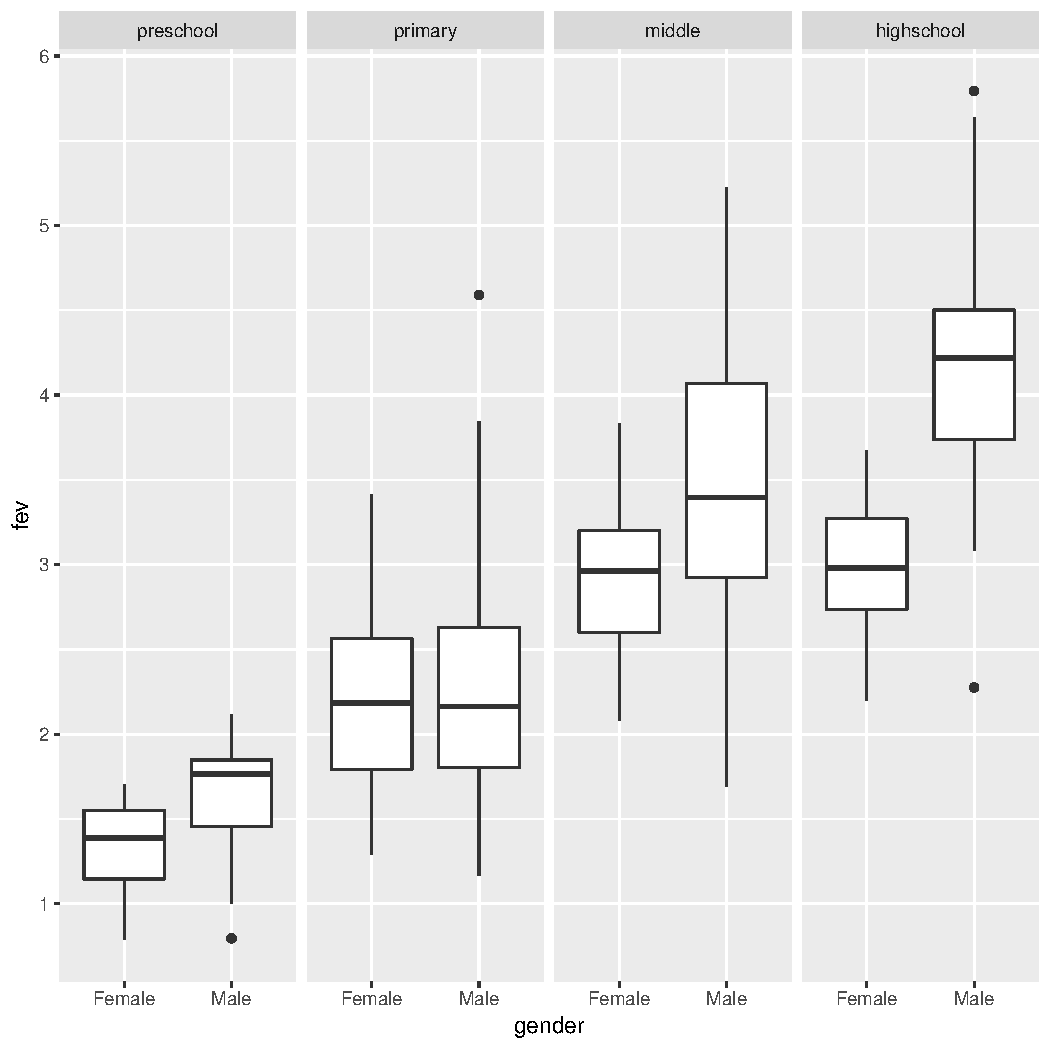
\includegraphics[width=\maxwidth,height=.6\linewidth]{figure/unnamed-chunk-4-1} 

}



\end{knitrout}
\end{frame}



\section{Histograms}

\begin{frame}[fragile]{Histograms by Gender}
\begin{knitrout}\footnotesize
\definecolor{shadecolor}{rgb}{0.969, 0.969, 0.969}\color{fgcolor}\begin{kframe}
\begin{alltt}
\hlcom{# initiate ggplot, specify breaks}
\hlstd{m} \hlkwb{<-} \hlkwd{ggplot}\hlstd{(fev,} \hlkwd{aes}\hlstd{(}\hlkwc{x} \hlstd{= fev))} \hlopt{+} \hlkwd{geom_histogram}\hlstd{(}\hlkwc{colour} \hlstd{=} \hlstr{"black"}\hlstd{,}
    \hlkwc{fill} \hlstd{=} \hlstr{"white"}\hlstd{,} \hlkwc{breaks} \hlstd{=} \hlkwd{seq}\hlstd{(}\hlnum{0}\hlstd{,} \hlnum{6}\hlstd{,} \hlnum{0.2}\hlstd{))}
\end{alltt}
\end{kframe}
\end{knitrout}
\pause
\begin{knitrout}
\definecolor{shadecolor}{rgb}{0.969, 0.969, 0.969}\color{fgcolor}\begin{kframe}
\begin{alltt}
\hlcom{# plot FEV by gender}
\hlstd{m} \hlopt{+} \hlkwd{facet_grid}\hlstd{(}\hlopt{~}\hlstd{gender)}
\end{alltt}
\end{kframe}
\end{knitrout}

\end{frame}


\begin{frame}[fragile]{Histograms by Gender}

\begin{knitrout}\footnotesize
\definecolor{shadecolor}{rgb}{0.969, 0.969, 0.969}\color{fgcolor}\begin{kframe}
\begin{alltt}
\hlstd{m} \hlkwb{<-} \hlkwd{ggplot}\hlstd{(fev,} \hlkwd{aes}\hlstd{(}\hlkwc{x} \hlstd{= fev))} \hlopt{+} \hlkwd{geom_histogram}\hlstd{(}\hlkwc{colour} \hlstd{=} \hlstr{"black"}\hlstd{,}
    \hlkwc{fill} \hlstd{=} \hlstr{"white"}\hlstd{,} \hlkwc{breaks} \hlstd{=} \hlkwd{seq}\hlstd{(}\hlnum{0}\hlstd{,} \hlnum{6}\hlstd{,} \hlnum{0.2}\hlstd{))}
\hlstd{m} \hlopt{+} \hlkwd{facet_grid}\hlstd{(}\hlopt{~}\hlstd{gender)}
\end{alltt}
\end{kframe}

{\centering 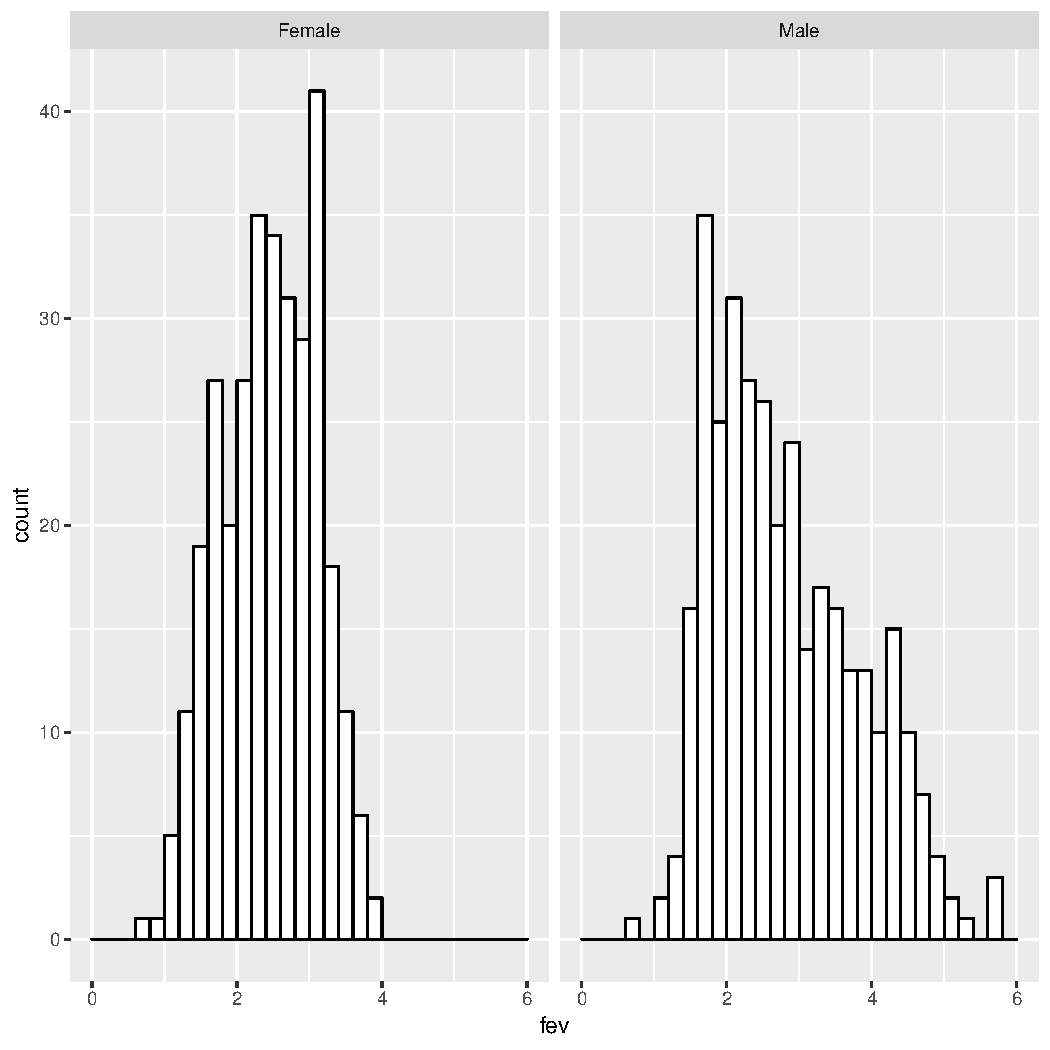
\includegraphics[width=\maxwidth,height=.6\linewidth]{figure/unnamed-chunk-7-1} 

}



\end{knitrout}

\end{frame}


\begin{frame}[fragile]{Histograms by Gender-Education Combinations}

\begin{knitrout}
\definecolor{shadecolor}{rgb}{0.969, 0.969, 0.969}\color{fgcolor}\begin{kframe}
\begin{alltt}
\hlcom{# where 'm' is the same as previous slide}
\hlstd{m} \hlopt{+} \hlkwd{facet_grid}\hlstd{(gender} \hlopt{~} \hlstd{edu)}
\end{alltt}
\end{kframe}

{\centering 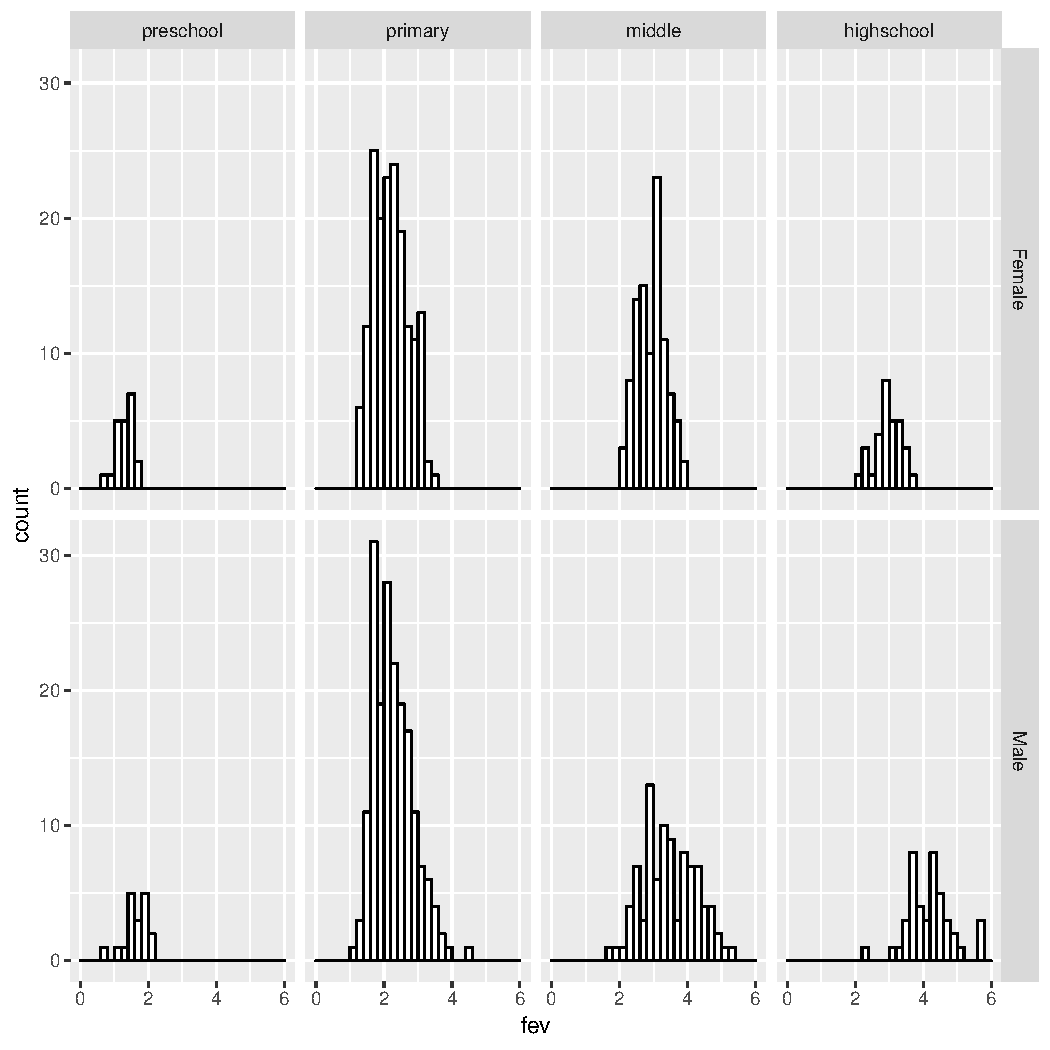
\includegraphics[width=\maxwidth,height=.6\linewidth]{figure/unnamed-chunk-8-1} 

}



\end{knitrout}
\pause
\textcolor{red}{Question:} \textit{What is the problem with this plot?}

\end{frame}


\begin{frame}[fragile]{Table of Gender-Education Combinations Counts}

\begin{knitrout}
\definecolor{shadecolor}{rgb}{0.969, 0.969, 0.969}\color{fgcolor}\begin{kframe}
\begin{alltt}
\hlkwd{xtabs}\hlstd{(}\hlopt{~}\hlstd{edu} \hlopt{+} \hlstd{gender,} \hlkwc{data} \hlstd{= fev)}
\end{alltt}
\begin{verbatim}
##             gender
## edu          Female Male
##   preschool      21   18
##   primary       168  183
##   middle         98   92
##   highschool     31   43
\end{verbatim}
\end{kframe}
\end{knitrout}

\end{frame}


\begin{frame}[fragile]{Density of Gender-Education Combinations}
To make the plots more comparable \textcolor{red}{plot their densities}
\pause
\begin{knitrout}
\definecolor{shadecolor}{rgb}{0.969, 0.969, 0.969}\color{fgcolor}\begin{kframe}
\begin{alltt}
\hlcom{# where 'm' is the same as previous slides}
\hlstd{m} \hlopt{+} \hlkwd{aes}\hlstd{(}\hlkwc{y} \hlstd{= ..density..)} \hlopt{+} \hlkwd{facet_grid}\hlstd{(gender} \hlopt{~} \hlstd{edu)}
\end{alltt}
\end{kframe}

{\centering 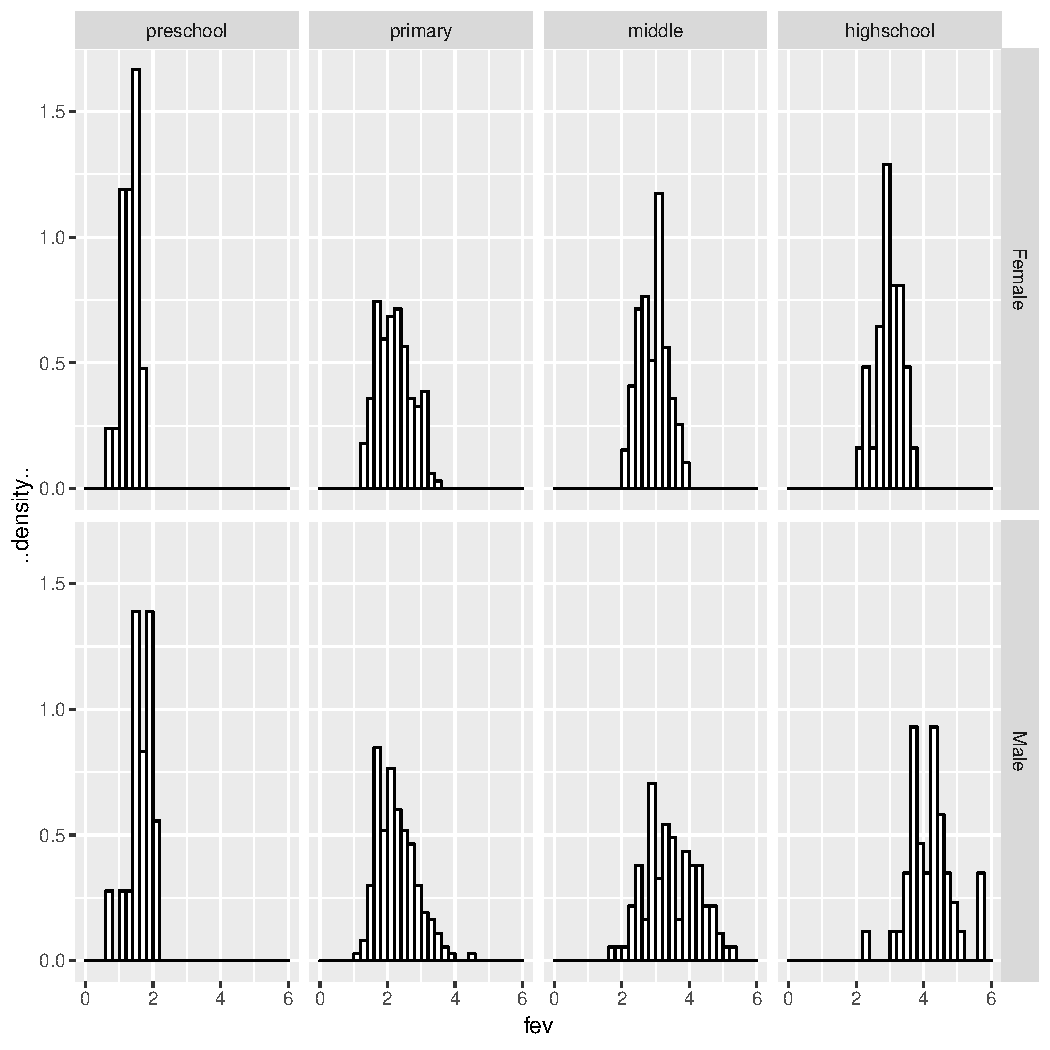
\includegraphics[width=\maxwidth,height=.6\linewidth]{figure/unnamed-chunk-10-1} 

}



\end{knitrout}

\end{frame}

\begin{frame}[fragile]{Histogram vs. Density of FEV}

\begin{knitrout}
\definecolor{shadecolor}{rgb}{0.969, 0.969, 0.969}\color{fgcolor}

{\centering 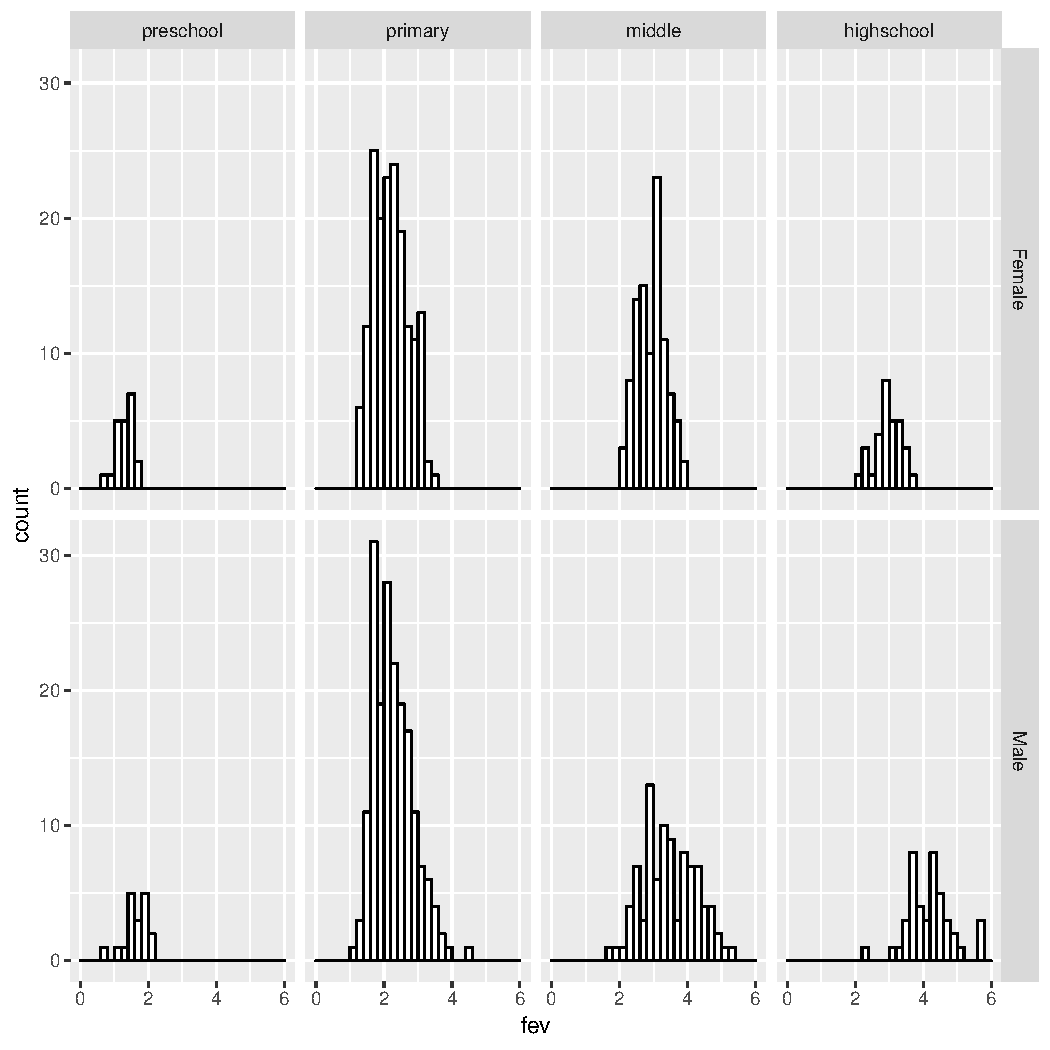
\includegraphics[width=\maxwidth,height=.4\linewidth]{figure/unnamed-chunk-11-1} 

}



\end{knitrout}

\begin{knitrout}
\definecolor{shadecolor}{rgb}{0.969, 0.969, 0.969}\color{fgcolor}

{\centering 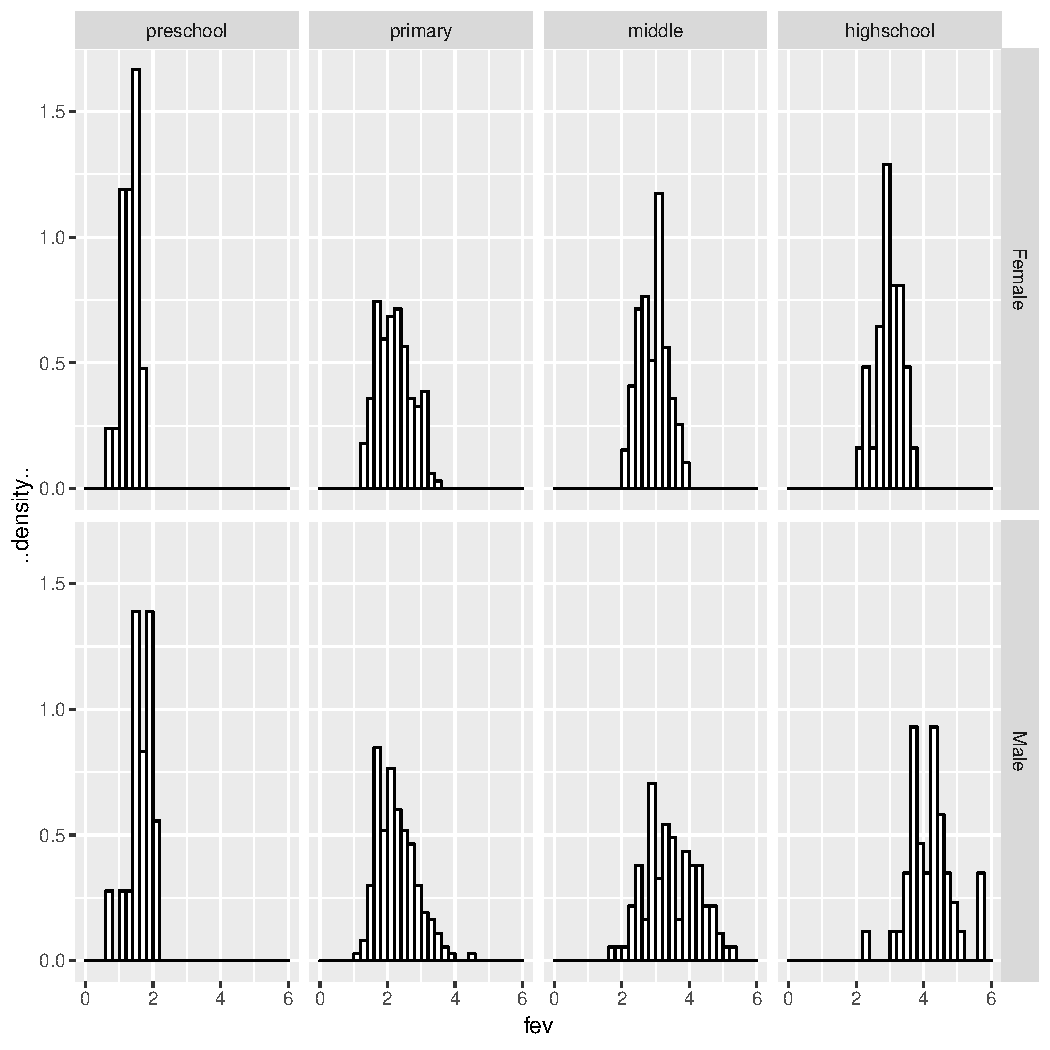
\includegraphics[width=\maxwidth,height=.4\linewidth]{figure/unnamed-chunk-12-1} 

}



\end{knitrout}


\end{frame}


\begin{frame}{References}
\small
\bibliography{005-bibliography}
\end{frame}


\begin{frame}[fragile]{Session Info}
\begin{knitrout}\footnotesize
\definecolor{shadecolor}{rgb}{0.969, 0.969, 0.969}\color{fgcolor}\begin{kframe}
\begin{alltt}
\hlkwd{print}\hlstd{(}\hlkwd{sessionInfo}\hlstd{(),} \hlkwc{locale} \hlstd{=} \hlnum{FALSE}\hlstd{)}
\end{alltt}
\begin{verbatim}
## R version 3.6.0 (2019-04-26)
## Platform: x86_64-pc-linux-gnu (64-bit)
## Running under: Pop!_OS 18.10
## 
## Matrix products: default
## BLAS:   /usr/lib/x86_64-linux-gnu/blas/libblas.so.3.8.0
## LAPACK: /usr/lib/x86_64-linux-gnu/lapack/liblapack.so.3.8.0
## 
## attached base packages:
## [1] stats     graphics  grDevices utils    
## [5] datasets  methods   base     
## 
## other attached packages:
## [1] ggplot2_3.1.0 plyr_1.8.4    knitr_1.22   
## 
## loaded via a namespace (and not attached):
##  [1] Rcpp_1.0.1       magrittr_1.5    
##  [3] tidyselect_0.2.5 munsell_0.5.0   
##  [5] colorspace_1.4-0 R6_2.4.0        
##  [7] rlang_0.3.4      highr_0.8       
##  [9] stringr_1.4.0    dplyr_0.8.0.1   
## [11] tools_3.6.0      grid_3.6.0      
## [13] gtable_0.2.0     xfun_0.6        
## [15] withr_2.1.2      lazyeval_0.2.1  
## [17] assertthat_0.2.1 tibble_2.1.1    
## [19] crayon_1.3.4     reshape2_1.4.3  
## [21] formatR_1.6      purrr_0.3.2     
## [23] glue_1.3.1       evaluate_0.13   
## [25] labeling_0.3     stringi_1.4.3   
## [27] compiler_3.6.0   pillar_1.3.1    
## [29] scales_1.0.0     pkgconfig_2.0.2
\end{verbatim}
\end{kframe}
\end{knitrout}
\end{frame}



\end{document}
